%!TEX root = ../thesis.tex
%2 - Tools for spectral analysis

\chapter{NIR spectroscopic reduction} % Main chapter title
\label{cha:reduction} 
%----------------------------------------------------------------------------------------
%	SECTION 1
%----------------------------------------------------------------------------------------
The work of this thesis relies on the use of {\nir} spectra obtained by the CRIRES instrument. This chapter contains an overview of the steps undertaken to extract astronomical spectra, focusing on the CRIRES instrument specifically. A comparison between the two reduction pipelines is performed. Detail of some issues we encountered with the reduction output are presented as well as the post reduction steps we performed, specifically wavelength calibration and telluric correction. The reduced spectra produced in this chapter will be used in \cref{cha:Chapter3} and \cref{cha:Chapter4}. We wrap up this chapter by highlighting other techniques in high resolution {\nir} spectra reduction and calibration which may have improved some of the results.  

\section{Summary of dataset}
\todo{}{}
Brief summary of dataset we focus reduction on. The motivation of these will be explained in \cref{cha:Chapter3}.

 
\section{NIR spectroscopy}
\todo{}{}
Specifics of {\nir} verse optical

NIR spectroscopy requires the use of CMOS detectors which are a different technology to the more commonly known CCD's. Their use is required in the {\nir} as the quantum efficiency (how well it measures photons) for CCD's although great for visible is poor in the \nir. CMOS detectors have a higher quantum efficiency in the \nir. 
\change{rearrange/reorganize this paragraph.}

CCD based on Silicon which doesn't work with \nir


\subsection{General reduction Concepts}
\label{subsec:nirreduction}
\unfinished{Should this general stuff be an appendix? }

Focus on our observations

There are 3 main effects that need to be accounted for in {\nir} spectroscopy which influence the observations and calibrations taken. We briefly detail them here and how they are corrected for

\begin{figure}[h]
\centering
%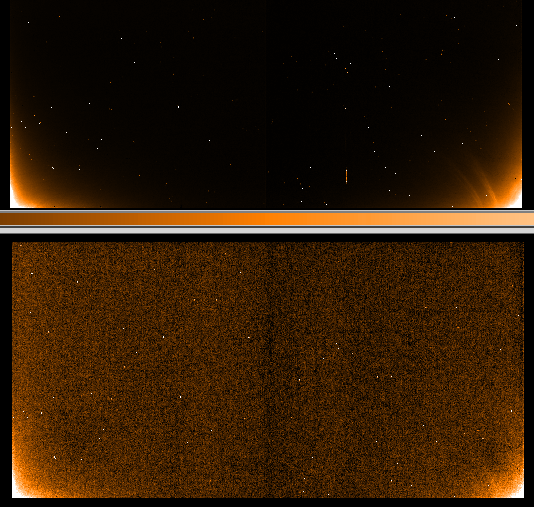
\includegraphics[width=0.4\textwidth]{figures/reduction/Master_Darks.png}
\includegraphics[width=0.9\textwidth]{figures/reduction/master_darks_1.pdf}
\caption{Master dark frames for exposure times of  3 and 180 seconds. Each master is created by averaging 3 images in which the detector received no incident light. Both frames are on the same scale and show dark current grows with exposure time. The color has been inverted so that black is the recorded measurement.}
\label{fig:darkcurrent}
\end{figure}

\subsubsection{Dark Current}
The dark current is a form of instrumental noise, in which the detector measures photons while not being illuminated. It is the detection of thermal electrons moving inside the detector, creating spurious photon counts. Calibration and removal of the dark current is performed by taking exposures in which the detector is not illuminated. 
 The temperature of the detectors in CRIRES instrument are kept at \textbf{XXX degree C} to significantly reduce, and to maintain consistent a low dark current. The electrical components of the CRIRES detectors create thermal energy while operational which impacts the dark current. A strong glow is observed in the bottom corners of the CRIRES detector in \fref{fig:darkcurrent} due to the presence of nearby amplifiers. As per the CRIRES calibration plan, ``dark frames'' need to be taken for each exposure time used. \fref{fig:darkcurrent} shows the master dark frame created from averaging three dark frames for exposure times of 3 seconds (for the flats) and 180 seconds (for the science), both on the same amplitude scale.
For the CRIRES detectors the dark current per pixel is around 0.2-0.4\,(\(e^{-}\)\si{\per\second}), while the glow at the two corners of the 180 second exposure shown here is around \(\sim9000 / 180\approx50\)\,\(e^{-}\)\si{\per\second}.


\begin{figure}[h]
    \centering
    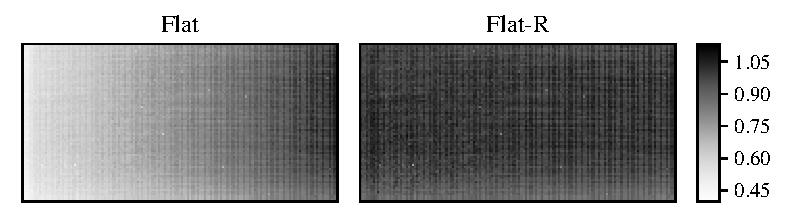
\includegraphics[width=0.9\textwidth]{figures/reduction/master_flats_1.pdf}
    \caption{A flat-field image for detector \#1 before (left) and after(right) the non-linearity corrections are performed. A perfect detector would have all pixels in the flat-field equal to 1. \bf{\red Remove flat and flatR titles.}}
    \label{fig:masterflats}
\end{figure}

\subsubsection{Flat-field}
No detector is truly perfect, with all pixels performing equally well. To correct for pixel-to-pixel variations in photon sensitivity across the detector and for any distortions in the optical path, a flat-field correction is needed. Exposures of a uniform\footnote{Ideally uniform intensity and spectral distribution} light source are taken, allowing the individual pixel-to-pixel sensitivity to be measured and corrected. The flat-field frames are corrected for dark current by subtraction of the master dark frame with the appropriate exposure time.

The CRIRES detector suffers from nonlinearities in sensitivity across the detector. This can be seen in the flat-field image on the left of \fref{fig:masterflats} where there is a gradient from white to black across the detector. A set of coefficients for each pixel is provided by ESO\footnote{Available at \href{https://www.eso.org/sci/facilities/paranal/instruments/crires/tools.html}{https://www.eso.org/sci/facilities/paranal/instruments/crires/tools.html}} to apply the correction for the nonlinearity of the detectors. This also corrects for a slight difference in sensitivity between the pixels from the odd and even columns in the CRIRES detectors, commonly called the ``odd-even effect''. The frame on the right of \fref{fig:masterflats} has been corrected for the nonlinearities.

\subsubsection{Nodding and Jitter}
The technique of \emph{nodding} is used to remove sky emission, detector dark current, and glow. First, an observation is spit into multiple separate exposures. Between each exposure the telescope is moved to change the vertical position of the target in the slit. The light from the star travels through a slightly different optical path and is recorded on a different part of the detector. The frames from the two nod positions (A, B) are then subtracted (A-B) to remove the background measurement from each spectra.

A visual example of the nodding is shown in \fref{fig:nodimages}. On the left are slices of 150 pixel columns from successive nod positions A and B as well as the difference A-B. On the right is a single pixel column from each image on the left. The background signal at the level of 20-30 counts in the image is almost canceled out by the opposite nod. This efficiently removes the background signal/noise from the observed spectra target. 

Observations of faint targets, that need long exposure times, are also broken up into multiple images so that the instrument glow from \fref{fig:darkcurrent} does not saturate the detector.

\begin{figure}
    \centering
    \begin{tabular}{cc}
        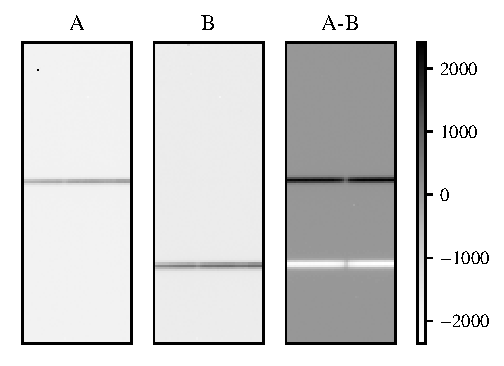
\includegraphics[width=0.4\textwidth]{figures/reduction/nod_image_sample.pdf} &
        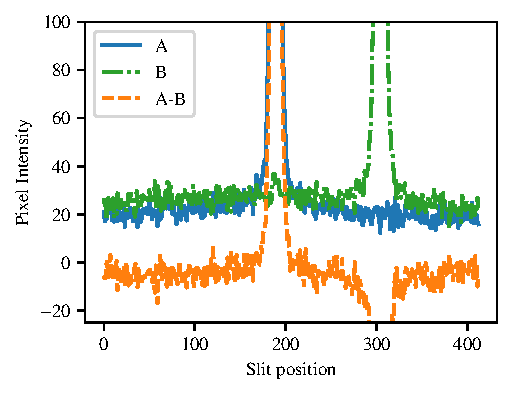
\includegraphics[width=0.37\textwidth]{figures/reduction/nod_slice_example.pdf}\\
    \end{tabular}
    \caption{Illustration of the nodding technique. Left: Sample slices of successive images at nod position A, B and their difference A-B for detector \#1. Right: A vertical slice along the slit at column 512 (middle of detector). The background level observed in A and B is effectively removed by the subtraction. {\red A and B backgrounds should be different on left. (just above zero ) and the spectra should be blacker, scale 2 A-B?}}
    \label{fig:nodimages}
\end{figure}

A small random vertical offset is applied to each observation which ensures that all spectra at the same nod position do not consistently land on the same pixels each time. This is known as the \emph{jitter} and allows for the correction of bad pixels and decreases the effect from any systematics of the detector.

\change{move}{As an example for the CRIRES observations analyzed for the main work here they were performed with an ABBAABBA nod cycle pattern with an exposure time of 180s each, or 24 minutes all up.}


\subsection{{\thar} lamp calibration}
As part of the CRIRES calibration procedure spectra are taken {\thar} lamps. The {\thar} spectra are placed into the instrument using 6 optical fibers, creating 6 uniformly spaced spectra across the detector.
\fref{fig:caliblamps} contains the {\thar} spectra for all four detectors, with the {\thar}. There are roughly 50 {\thar} lines that fall across the four detectors for the wavelength setting here, although most of them are quite faint, With the scaling shown in these images only around 10 of the brightest lines can be just detected by eye. 

The purpose of these fibers is to cross-correlate each with a {\thar} template, obtaining a wavelength solution across the detector. Scratches on the detector can cause a decrease in the correlation between {\thar} lines and the spectral template in ESO pipeline. This can be resolved by first applying a pixel mask (although we did not attempt it). At the top and bottom there are also 2 meteorological fibers that can not be used for wavelength calibration as they pass through a different optical pathway.  The brightest one at the bottom seems to have strong features that overwhelm or washout many columns in detector 2--4 (vertical stripes). \unfinished{Check if it is mentioned how these get corrected/ if the impact the wavelength solution.}
In the end we did not use the {\thar} calibrations, this is discussed in \sref{subsec:wavecalib}. They have still been included here for completeness.

\begin{figure}
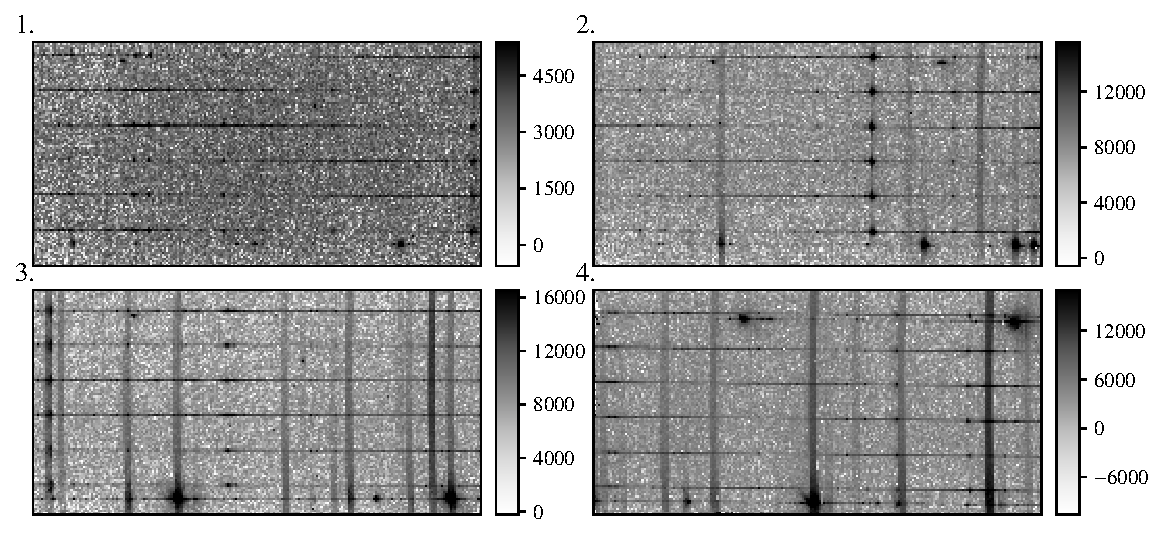
\includegraphics[width=\hsize]{./figures/reduction/lamp_plots_cbar_each.pdf}
\caption{A Th-Ar calibration lamp frame for each detector, corrected from the dark current.}
    \label{fig:caliblamps}
\end{figure}

\todo{Note: Useful information about MIR reduction in the 
\href{https://www.eso.org/sci/facilities/paranal/instruments/visir/doc/VLT-MAN-ESO-14300-3514_2018-02-01.pdf}{VISIR manual}}

\subsection{Extraction}
Basically counting the photons in a narrow region about the spectrum. Order tracing is done to follow any curvature in the spectrum...
optimal / rectangular...
\missingfigure{Sketch of order tracing?}

There are two types of extraction commonly used. The \emph{rectangular} extraction performs a rectangular aperture sum in the spatial direction while the \emph{optimal} extraction~\citep{horne_optimal_1986} also includes variance weighting to reduce the impact of the noise and deviant pixels on the total flux measurement. Optimal extraction is the most common and is the default output of both the ESO and DRACS pipelines.

\section{Pipeline Comparison}
\change{Reword}{To be able to extract the target spectra from the calibration and observation images a number of steps, some outlined above in \sref{subsec:nirreduction}, have to be performed in sequence. }The series of steps, performed by various software tools, is referred to as a \emph{pipeline}. Each stage in the pipeline performs a specific task, for example, creating the master dark frame or performing the nod subtraction). The result of one stage is passed to the next (automatically or manually). Two different pipelines were available to reduce the CRIRES observations used in this work. The first is the standard CRIRES pipeline\footnote{\href{https://www.eso.org/sci/software/pipelines/}{https://www.eso.org/sci/software/pipelines/}}, available from ESO.
The second is an in-house pipeline originally \change{was this the first instance} used in~\citet{figueira_radial_2010} called DRACS (Data Reduction Algorithm for CRIRES Spectra) \change{Pedro it is my understanding that the ESO pipeline did not exist/was not available when you created DRACS, correct?}

In these next sections we document our experience using both pipelines, and compare the extracted spectra and user experience.

ESO has a new reduction ``workflow'' called EsoReflex, it is not available for CRIRES, and not expected to be ever supported.

\subsection{CRIRES pipeline}
The spectra were initially reduced using the ESO CRIRES pipeline \href{ESO CRIRES pipeline}{ESO CRIRES pipeline}. The \href{https://www.eso.org/sci/software/gasgano.html}{GASGANO} graphical user interface (GUI) for the pipeline was used. The CRIRES reduction cookbook\footnote{\href{https://www.eso.org/sci/facilities/paranal/instruments/crires/doc/VLT-MAN-ESO-14200-4032\_v91.pdf}{https://www.eso.org/sci/facilities/paranal/instruments/crires/doc/VLT-MAN-ESO-14200-4032\_v91.pdf}} was followed to reduce the CRIRES nodding spectra. The CRIRES pipeline user manual\footnote{\href{ftp://ftp.eso.org/pub/dfs/pipelines/crires/crire-pipeline-manual-1.13.pdf}{ftp://ftp.eso.org/pub/dfs/pipelines/crires/crire-pipeline-manual-1.13.pdf}} and the GASGANO manual\footnote{\href{here}{here}}. The pipeline provides a number of \emph{recipes} which perform the required extraction steps. From the GUI each recipe is manually selected, then the correct calibration and observation files are selected and added. 
\begin{itemize}
\item - dark creation
\item - flat creation
\item - wavelength calibration
\item - jitter extraction
\end{itemize}

The wavelength calibration was the most tedious. To try and improve the wavelength calibration the y positions of the 6 {\thar} fibers was found for each detector and entered into the parameters for each observation. This sometimes helped but not always in the end we did not use them anyway.

The final output is a extracted and flattened spectra (although not normalized to 1) both in a rectangular and optimal and errors, with a wavelength calibration.

\textbf{Opinions: SHOULD I BE including my opinions on the usage?}
DONT READ Just unsorted junk: 

\textit{- For the extraction of many spectra it soon became tedious. Having to tweak parameters to obtain a better reduction. Then having to remember and change for each observation. }

\textit{- Having the available options visible in the GUI for each spectrum is handy if you need to change them.}



\textit{One good thing is it had the list of parameters available to tweak for that recipe visible..}

\textit{It is believed that there is a way to enable batch processing???}

\textit{It soon became tedious to use the Gasgano GUI to extract the many spectra reduce many and tweak all the parameter settings manually. In particular manually measuring and adding the vertical positions of the 6 {\thar} lines for each detector and observation. This was in an attempt to improve the wavelength calibration provided by the {\thar} lamp spectra.
A number of other parameters were tweaked from the defaults in an attempt to improve the reduction. Again become tedious to repeatably change the parameters for all observations.}

\textit{Having the GUI did however allow for a easy introduction into using performing spectral reduction when not of not yet comfortable with the command line (required for the ESOREX interface).
There is a command line interface available, ESOREX but it is not The newer ESO pipeline reduction tool Reflex does not have a pipeline for CRIRES. }


\subsection{DRACS}
DRACS (Data Reduction Algorithm for CRIRES Spectra) is custom reduction pipeline~\citep{figueira_radial_2010} written in IRAF's CL\footnote{IRAF is distributed by the National Optical Astronomy Observatories, which are operated by the Association of Universities for Research in Astronomy, {Inc.}, under cooperative agreement with the National Science Foundation.}~\citep{tody_iraf_1993}. It provides for automated dark and nonlinearity corrections (using the nonlinearity coefficients provided by ESO), as well as the flagging and replacement of bad pixels. The images are corrected from sensitivity variations by dividing by a flat-field corrected from the blaze function effect. The nodding pairs are mutually subtracted and the order tracing is accomplished by fitting cubic splines
Order tracing allows the extraction algorithm to follow the shape for the dispersion across the detector \unfinished{is footnote  correct "instruments optics"}\footnote{The spectra do not fall perfectly horizontally on the detector and usually contain some curvature due to the instruments optics.}. 
By default the pipeline returns the \emph{optimal }extraction~\citep{horne_optimal_1986}, but the \emph{rectangular} extraction can also be obtained. (see \sref{subsubsec:reductionartifacts} for more details).
The extracted spectra from each nod is continuum normalized by dividing by a polynomial fitted to the continuum, with the polynomial degree selected for each spectrum and detector. Finally the normalized nod-cycle spectra are averaged together to give a single reduced spectrum, normalized to 1.

The DRACS pipeline was originally developed to work with H-band spectra, some internal parameters were adjusted slightly in an attempt to achieve a better reduction on the K-band spectra analyzed here.


Opinions:
DONT READ UNFINISHED 

\textit{The DRACS can be run semi-autonomously so that it provides a consistent reduction relatively easily. It remembers the order tracing and}

How to use:
\textit{To use DRACS you need to create a number of lists with different, darks, flats, observations\footnote{The GASGANO GUI was helpful to help identify the distinction of each fits file for a beginner}. A similar process with list of files is done with the ESOREX pipeline.}
\textit{Once these list are created then the main script can be executed that semi-autonomously performs the reduction. The first time though there are a number of manual checks/decisions, (e.g. confirming the order tracing position, and fit) but DRACS remembers them. This means the extraction requires less manual input if run a second or third time though.}

\textit{This was handy when trying to tune some of the internal parameters to perform a better extraction.}

\missingfigure{Order tracing example plot?, exaggerated sketch} 

\textit{The most tedious thing about DRACS is creating the lists for the different input parameters}

\textit{This semi-autonomous nature mean all the spectra are reduced in a consistent way and quickly, not requiring manual spectra selection for each observation.}


\subsection{Pipeline comparison and selection}

Both reduction methods were applied to the same CRIRES spectra to check for consistency and quality of both methods. \fref{fig:reductioncomparsion} shows the reduced spectra from both methods\ldots.

One of the important things we checked was the line depth of the spectra. To insure that DRACS was comparable to the ESO pipeline.
\missingfigure{Some spectra from both reduction methods to show similarities, }
\begin{figure}
   \label{fig:reductioncomparsion}
\end{figure}

We in-fact found they were the same line depth.


After using both it was decided to continue using DRACS \ldots for this reasons

With these considerations at this point we decided to perform the rest of the reductions with the DRACS pipeline. This would require a manual wavelength calibration to be performed. 


BUT: We eventually found some strange inconsistencies in the DRACS reduction, artifacts. where bad pixels were non-optimally corrected\ldots.
In hindsight it may have been better to use ESO (if a way to semi-automation was discovered)

\subsubsection{Reduction issues}
\label{subsubsec:reductionartifacts}
\TODO{Check optimal extraction parameters, may have reduced the extraction width by too much?? Need to check changing it.}
At a later date some large artifacts in the DRACS extracted spectra were identified. An investigation in to the cause of these artifacts was undertaken to identify their source and remove them from the spectra. Separating out the individual nod spectra side-by-side revealed that the artifacts were occurring in only a few of the individual nod spectra from the optimal extraction and that they were not present in the rectangular extracted nods. Four examples are shown in \textbf{Figures ..blah an blah.} In each panel the top sub-plot contains the optimal extracted spectra, while the middle sub-plot contains the rectangularly extracted spectra.

It is is obviously clear that the artifacts in the optimal nod correspond to large bad pixel spikes present in the rectangular extracted nod. The difference between the rectangular and optimal extraction is that the optimal is the rectangular extraction but weighted by its variance. It appears that the presence of cosmic rays or bad pixels heavily affected the variance weighting during the \emph{optimal} extraction. It is also observed that the artifact creates are not localized to the bad pixel region but affect a large spectral range (100's of pixels in some cases). 

The artifacts were observed to create flux deviations in the fully combined optimally extracted spectra of \(\sim 0.5\% \). Therefore, we took measures to remove these artifacts before combining the nod spectra as the science case for these observations is to recover companion spectra with expected flux ratios \(\rm {F_2}/{F_1} < 1\% \). 

Numerous parameters in the DRACS were experimented with to try and remove the observed artifacts with no success. We therefore decided to replace the optimally extracted nods that had artifacts with their rectangular counterparts. 
An iterative 4-\(\sigma \)\footnote{There is no justification why 4-\(\sigma\) was chosen over the commonly used 3-\(\sigma\).} rejection algorithm\footnote{Found at \url{https://github.com/jason-neal/nod_combination}} was applied to the replacement rectangular extractions to remove the erroneous pixels that caused the artifacts. The \(\sigma\) value for each pixel was calculated as the standard deviation of the nearest 2 pixels on either side of all 8 nod spectra. Any rejected pixels were replaced using linear interpolation.

We note that we did not really observe a pattern in which nod, and in which position were going to be artifacts. there are many other spikes in the rectangular extractions that do not create the artifacts observed. 

Combined spectra were finally constructed by averaging the 8 nod-cycle spectra together, where some of the optimally extracted spectra have been replaced using the above method. The last panels of \fref{fig:nodartifacts} shows that the difference between the combined spectra using only optimally extracted spectra and the combination with replacements.
\todo{Do the figures}

\begin{figure}
    \centering
    \begin{tabular}{cc}
    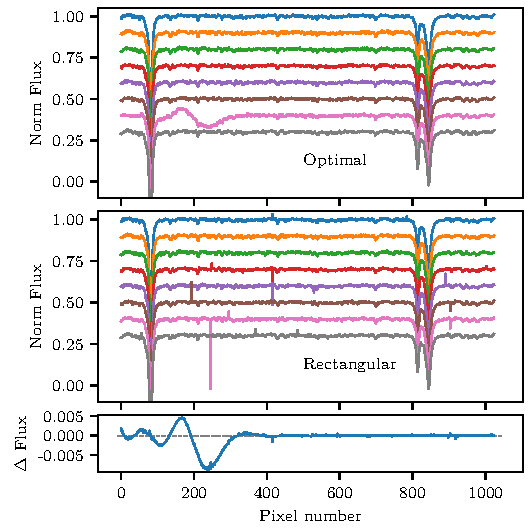
\includegraphics[width=\hsize/2]{figures/reduction/Bad_pixel_replacement} &
    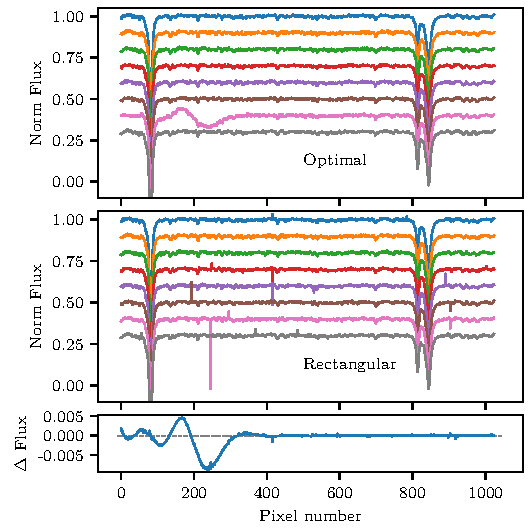
\includegraphics[width=\hsize/2]{figures/reduction/Bad_pixel_replacement}\\
     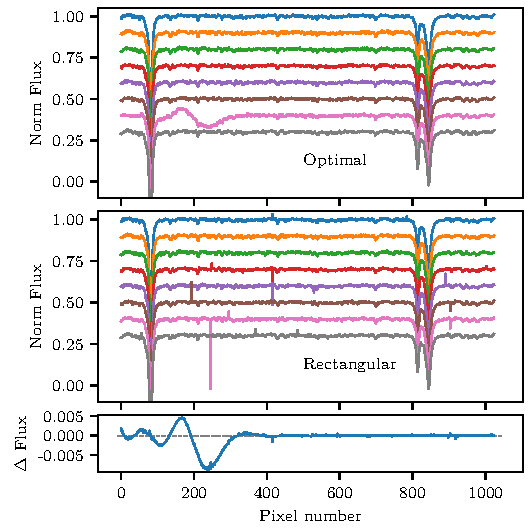
\includegraphics[width=\hsize/2]{figures/reduction/Bad_pixel_replacement} & 
     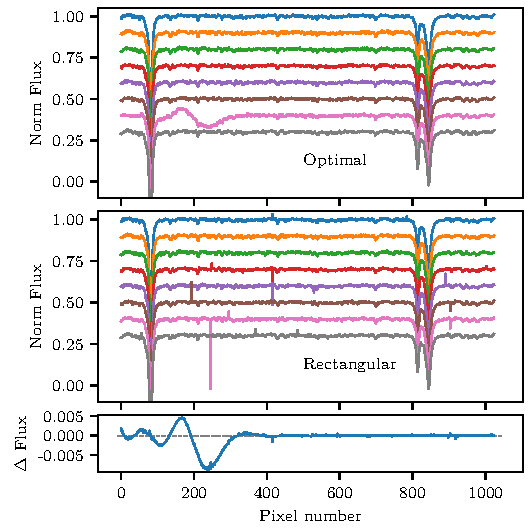
\includegraphics[width=\hsize/2]{figures/reduction/Bad_pixel_replacement}
     \end{tabular}
    \caption{Example of an artifact in the optimally extracted spectra. The top panel contains the 8 normalized nod spectra after optimal extraction, while the middle panel shows the rectangular extraction for the exact same spectra. A vertical offset is included between each spectra. For the first panel a single large spike in the seventh nod (pink) near pixel 230 creates a wide and noticeable artifact in the optimal extraction. The bottom panels shows the difference between a combined spectrum using optimal nods only and a combined spectrum in which the identified nods are replaced with their rectangular counterparts. The nod spectra are in observation order from top to bottom.  \textbf{this is obs ... detector x in which nod 7 is replace.}}
    \label{fig:badpixelreplacement}
\end{figure}


% Table of nods optimally reduced replaced by rectangular extraction and bad pixel replacement.
%!TEX root = ../thesis.tex
% Table of nods replaced for correction. 
\change{Maybe transpose \tref{tab:nod_replacement} to be shorter?}{}
\change{CHANGE \# into the ESO identification number 1b 2a etc}
\begin{table}
    \caption{Identification of all the optimally reduced nod spectra which had artefacts that were replaced by the rectangular extractions, corrected for bad pixels. The numbers represent the position in the nod cycle ABBAABBA. The number of the observation for each target is given by \#.}
    \label{tab:nod_replacement}
    \centering
    \begin{tabular}{cccccccc}
        \toprule
      & & \multicolumn{4}{c}{Detector}& \\
         Target  & \#  & 1 & 2 & 3 & 4 & Total \\ 
        \midrule
        \object{HD 4747}   & 1 & 8 & 5, 8 & 8 & 1, 5, 8 & 7\\
        \object{HD 162020} & 1 & - & 7, 8& - & - & 2\\ 
        \object{HD 162020} & 2 & - & 2 & - & 8 & 2\\ 
        \object{HD 167665} & 1 & 2, 4 & 8 & 1, 6 &  4, 5 & 7\\ 
        \object{HD 167665} & 2 & 2 & 3 & 1 & 8 & 4\\ 
        \object{HD 167665} & 3 & 6 & 3, 7 & - & 8 & 4\\ 
        \object{HD 168443} & 1& - & - & - & 7, 8 & 2\\ 
        \object{HD 168443} & 2 & - & 2, 4 & 6 & 8 & 4\\ 
        \object{HD 202206} & 1 & - & 6, 7& 1& - & 3\\ 
        \object{HD 202206} & 2 & 5 & - & 7,8 & - & 3\\ 
        \object{HD 202206} & 3 & 8 & 3 &  6 & 6 & 4\\ 
        \object{HD 211847} & 1 & - & 5, 7 & 2 & 4 & 4\\ 
        \object{HD 211847} & 2 & 2 & 1, 7 & 7 & 8 & 5\\ 
        \object{HD 30501}  & 1 & 7 & 7 & - & 8 & 3\\ 
        \object{HD 30501}  & 2 & 7, 8 & 3, 5, 7, 8 & 2, 7 & 2, 3&10 \\ 
        \object{HD 30501}  & 3 & 4, 8 & 2, 6, 7& 4, 8 & 7& 8\\ 
        \object{HD 30501}  & 4 & 1, 2, 4 & 3 & 5, 6 & 6 & 7\\
         \midrule
            &&&&&& 79/544\\
    \bottomrule
    \end{tabular} 
\end{table}

The normalization and nod combining steps were also performed using IRAF while the following post reduction procedures and analysis all utilize \emph{Python}. This pipeline was chosen over the ESO CRIRES pipeline because it seemed relatively simple to use, being mostly automated, and appeared to have less bad pixel/cosmic ray artifacts in the resulting spectra. In hindsight this was not the case, with artifacts appearing that needed to be removed. 

One possible explanation for the artifacts present is an instrumental effect, such as instrument glow. This is known to affect CRIRES and included in the data reduction cookbook~\citep{smoker_very_2012}. These artifacts in the K-band spectra were not observed in previous works in the H-band using this pipeline and as such may have a wavelength dependent affect, as the higher wavelength {\nir} is more susceptible to thermal instrument glow.



\textbf{In the paper We say it could be glow. I do not think it is anymore and think it is just bad pixels not correctly removed. Either way it does not affect our results significantly....
This method is likely to have a slight negative impact on the noise/snr.}

It could be that these are a incorrect bad pixel mask.


Note for HD202206 the 1st two nods have a much higher extracted flux. I am still unsure why this is...


\section{Reduction experience:}
The experience gained in reducing CRIRES spectra enabled participation in collaboration with other science cases. The DRACS pipeline was used to extract the spectra of two other targets. A target and a very brief aim of each science case is given below.
\begin{itemize}
\item Barnard's Star\footnote{Programme ID: 085.D-0161(A)}: The reduced {\nir} spectra of Barnard's Star was meant to extend the work of~\citet{andreasen_nearinfrared_2016} in deriving the spectroscopic parameters in the \nir. Unfortunately in the end the already reduced CRIRES-POP library was used instead in~\bf{citet{Andreasen et al. (in prep.)}}. \unfinished{reason}{This was because \ldots}
\item $\eta$ Tel\footnote{Programme ID: 083.C-0759(A)}: The spectra of $\eta$ Tel, quickly rotating Brown Dwarf, was reduced to accurately determine its rotation rate by measuring the line broadening. \change{}{Hagelberg et al. (in prep.)}
\item The same spectra of $\eta$ Tel were also used in~\citet{ulmer-moll_telluric_2018} to compare different telluric correction methods in the \nir.
\end{itemize}

For these works only the spectral extraction outlined above was performed. The post \change{I seem to use these interchangeably. are they}{extraction/reduction} steps from the following sections were not.

\missingfigure{An image of some reduced spectra from eta Tel and Barnard's star???}

\section{Post reduction stages}
\label{sec:posreduction}
From the DRACS pipeline we have extracted the 1-D spectra of each target. The spectra still need to undergo some post-reduction step. In particular, wavelength calibration and telluric correction. A detailed look of how these steps were developed and performed are addressed in the following section.

\subsection{Wavelength calibration}
\label{subsec:wavecalib}
Wavelength calibration is the process of assigning accurate wavelength values to each pixel in the spectra. For CRIRES in the {\nir} this is challenging. CRIRES uses a Thorium-Argon (\thar) lamp to place 6 emission spectra on the detector using fibers. The spectra of the {\thar} emission lines are used to determine the spatial distribution of the wavelength solution across each detector using correlation with a spectral template. \change{fix-up get a good citation, number of lines}{}{\thar} lamps are excellent at optical wavelengths where the numerous (8600 espresso) spectral lines enable precision of sub-m/s radial velocity measurements HARPS spectrograph\reference{paper for harps {\thar} lines}{(?)}. However in the {\nir}, there is a relatively low density of {\thar} lines~\citep{kerber_laboratory_2009}, which, in combination with the alignment of the narrow wavelength range of the detector, causes a poor wavelength calibration to be obtained (e.g.\ CRIRES-POP~\citep{nicholls_crirespop_2017}).
Above 2.2~\si{\micro\meter} there are {O-H} sky lines that can be used for wavelength calibration but for our observations below 2.2 \si{\micro\meter} they are too dim.\reference{ cite crires manual, a paper about sky lines?}

These wavelength calibration issues were experienced when using the ESO CRIRES pipeline, with non-Th-Ar lines features sometimes affecting the correlation.

At the wavelength of 2.1-2.17~\si{\micro\meter} there are roughly XXX {\thar} lines across all four detectors, as seen in \fref{fig:caliblamps}.
The DRACS pipeline does not use the {\thar} lamp files for wavelength calibration and leaves this as a post reduction step.

A common method for wavelength calibration that does not rely on Th-Ar lamps of CRIRES involves using the telluric lines present to provide the wavelength solution ~\citep[e.g.][]{brogi_signature_2012,brogi_carbon_2014,dekok_detection_2013}{\red piskorz2016}. This is made possible by the use of high resolution spectra, in which the telluric lines are well resolved, as well as accurate spectral information of the atmosphere. 

We follow this method using the telluric absorption lines present in each observation as the wavelength reference. Instead of directly using the HITRAN database~\citep{rothman_hitran2012_2013} for the telluric line positions \citet[such as in ][]{brogi_signature_2012,brogi_carbon_2014,dekok_detection_2013}), we use the TAPAS atmospheric transmission models~\citep{bertaux_tapas_2014} obtained for each observation. The TAPAS models in turns use the HITRAN database but includes atmospheric profiles and physical meteorological measurements to model the telluric absorption strength.

To calibrate the wavelength the telluric lines in the model need to be associated to the corresponding telluric lines in the observed spectrum. The centroid\footnote{Center of the line} of each telluric line in the model is obtained by fitting the telluric transmission spectrum, \(T(\lambda) \), as a simple sum of Gaussian functions (subtracted from the continuum).

\begin{equation}
T(\lambda) = 1 - {\Sigma}_{i}\ G(\lambda, A_{i}, {\mu}_{i}, {\sigma}_{i}),
\end{equation}

where \(G \) is a Gaussian function of the form

\begin{equation}
G(\lambda, A, \mu, \sigma) = {A \textrm{e}}^{{-(\lambda-\mu)}^{2}/2\sigma^{2}}
\end{equation}

and \(A \), \(\mu \), \(\sigma \) are the amplitude, central wavelength, and standard deviation for each line respectively. Telluric lines actually have a Voigt profile\footnote{A Voigt profile is a convolution of two broadening profiles, a Gaussian and a Lorentzian. Gaussian broadening results from thermal Doppler broadening, and instrumental broadening while the Lorentzian broadening comes from molecular vibrational bands\citep{meier_art_2005}.} but at this resolution the Gaussian profile dominates, and as such the Gaussian assumption is a sufficient to fit the line centers.

The observed spectra contain two different spectral components: stellar and telluric lines overlapped. This overlapping is, in fact, a multiplication of the stellar and telluric spectra. The observed spectra are fitted with two Gaussian-sum models multiplied together. The identification between telluric and stellar lines is performed manually for each spectra, using the telluric model as the reference. Care was taken to fit the correct components to blended spectra where possible to improved the number telluric lines use for calibration. The fits were inspected to ensure that they reasonably matched the line positions. There was difficultly in identifying the shallow lines with depths below 1-2\%. But these were needed in some spectra to obtain a suitable fit. 

\begin{align}
I_{obs}(x) &= I_{tell}(x) \times I_{space}(x) \nonumber \\
I_{obs}(x) &= \Big(1 - {\Sigma}_{j}\ G(x, A_{j}, {\mu}_{j}, {\sigma}_{j})\Big)_{tell} \times \Big(1 - {\Sigma}_{k} G(x, A_{k}, {\mu}_{k}, {\sigma}_{k})\Big)_{space}, \label{eqn:obs}
\end{align}

where \(x \) is the pixel coordinates of the extracted spectra.

\missingfigure{example figures illustrating this method}

After fitting \(I_obs(x)\) to the observed spectrum and \(T(\lambda)\) to the telluric model the wavelength solution was obtained by fitting a second order polynomial to the centroid values \(\{\mu_{j}(x), \mu_{i}(\lambda)\} \) from the telluric components of the observed spectra and telluric model respectively. A second order polynomial has been shown to be sufficient for higher precision RV studies~\citep[e.g.][]{bean_groundbased_2010, figueira_radial_2010}. This polynomial is then used to map the whole spectrum from pixels into wavelength values.

\missingfigure{Example of coordinates and the fit. Ca I calculate some errors on the polynomial coord fit.}

Much like with the {\thar} calibrations, this technique performs better when there is sufficient coverage of telluric lines on the detectors. For the wavelength setting of these observations, the spectra from the second detector (top right panel of \fref{fig:detector4allspectra}) only have two large telluric lines present with several small lines, with relative depths smaller than 1\%, which are often difficult to accurately identify. This deteriorated the calibration stability for the second detector. With the lack of telluric contamination and stellar lines on the second detector it may have been ideal for the detection of a faint secondary spectra; unfortunately the wavelength calibration quality varies in an inverse way.


We note that there are many variations on this wavelength-calibration technique including those integrated within programs such as TelFit~\citet{gullikson_correcting_2014}, and ESOs Molecfit~\citet{smette_molecfit_2015}, that perform telluric correction and re-calibrate the wavelength axis themselves at the same time.


A brief attempt of wavelength calibration using an iterative method outlined in \cite{brogi_rotation_2016}. This involved generating set of wavelength solutions for the observed spectrum, cross-correlating each one against the telluric model. The solutions for the next iteration are obtained by refining the parameters from the solution with the highest correlation. 
The method worked well for \citet{brogi_rotation_2016} as they included templates for both star and telluric lines were observing in a wavelength domain in which there is a large number of strong and uniform stellar CO lines across the detector. 
Our experiments with this method were not successful as we did not include a stellar mask or model. Without adding any stellar masking the telluric lines would strongly correlate to the stellar lines present, especially were there was blended lines. The lead to incorrect wavelength solutions This method was abandoned, but may have been possible if a stellar mask was used.

\missingfigure{Would a table of polynomial wavelength solutions along with errors be any use?}

\unfinished{Add pictures of wavelength calibrations}

\missingfigure{Extracted, normalized and wavelength calibrated spectra for a single observation of each target. The target name is given above each spectrum along with the observation number. Each panel is the spectra from a single detector 1--4 in order of increasing wavelength. The black dashed lines indicate the unique telluric spectrum used for wavelength calibration and telluric correction for each observation.}
% \begin{figure*}
% 	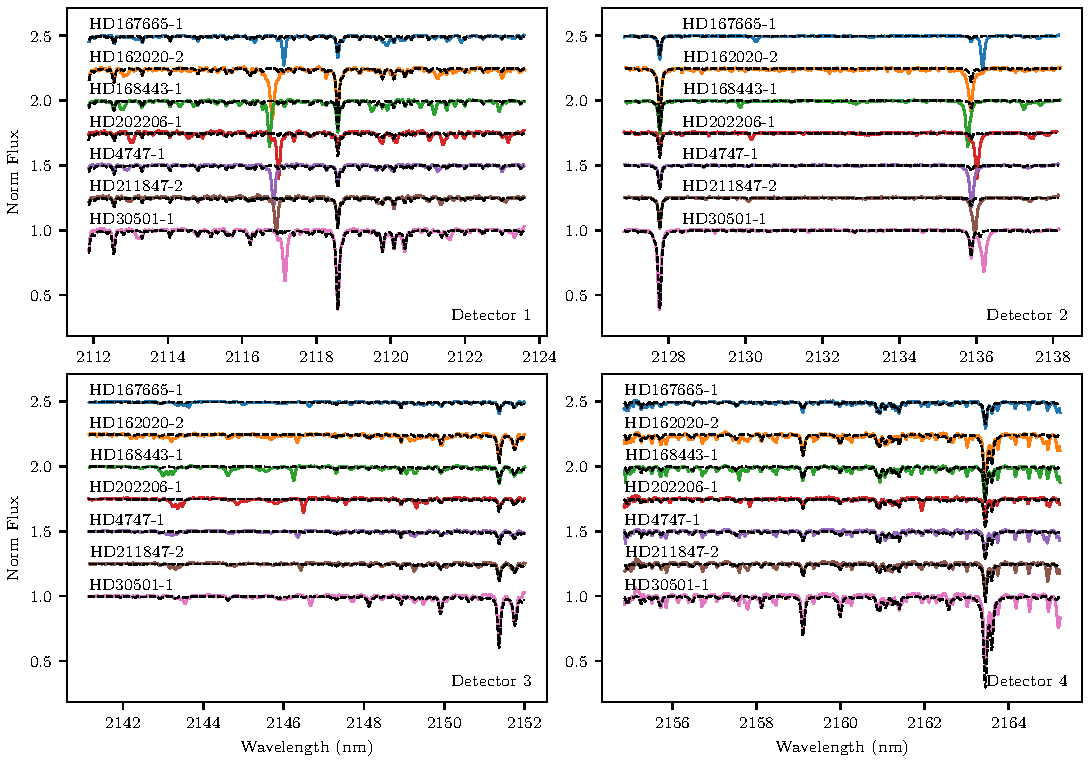
\includegraphics[width=\hsize]{figures/reduction/Spectra_examples.pdf}
% 	\caption{Extracted, normalized and wavelength calibrated spectra for a single observation of each target. The target name is given above each spectrum along with the observation number. Each panel is the spectra from a single detector 1--4 in order of increasing wavelength. The black dashed lines indicate the unique telluric spectrum used for wavelength calibration and telluric correction for each observation.}
% 	\label{fig:detector4allspectra}
% \end{figure*}

In the future it may be plausible to combine all of the methods above, including the Th-Ar calibration lines, telluric models, and stellar templates. Also applying a fit to the 4 detectors so that neighboring detectors can help with the fit when low lines are used.

\begin{figure}
    \centering
    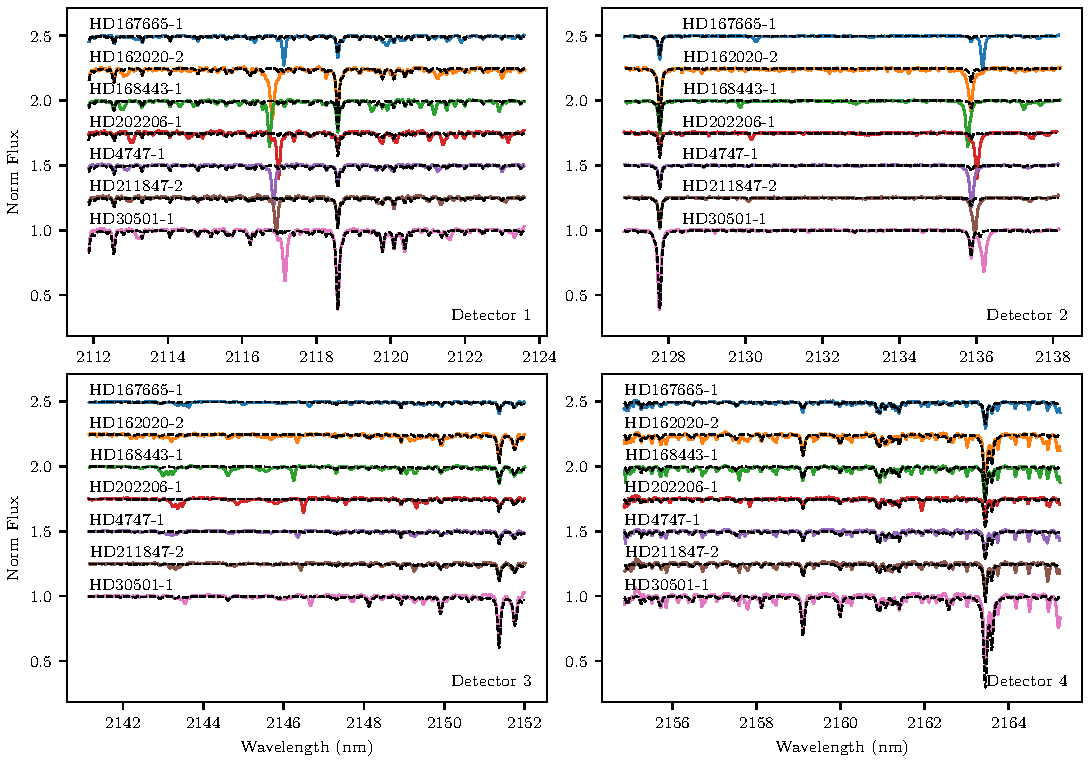
\includegraphics[width=1\linewidth]{figures/reduction/Spectra_examples}
    \caption{An example spectra for each target and detector. The solid lines are the spectra while the black dashed lines are the telluric models used for wavelength correction, showing good alignment with the spectra.}
    \label{fig:spectraexamples}
\end{figure}


\missingfigure{comparision between a gasgano wavelength solution and the manual one. This has not be done by me before... }



\unfinished{See Solene's paper regarding Telluric correction with models and reference spectra}

\subsubsection{Telluric correction}
\label{subsec:telluric_correction}
The Earth's atmosphere is a spectral filter for all ground-based astronomical observations, imprinting the absorption profile of the atmosphere onto the spectrum observed. To accurately recover the spectra of the observed target the removal of the absorption lines introduced by Earth's atmosphere is extremely important. The motion, changing composition and \todo{See solenes paper for matereial here}.
A number of methods are available to correct for the telluric lines, telluric reference (cite) , models (tapas), modeling/fitting (molecfit tellfit). The effectiveness between these three methods has recently been performed in \cite{ulmer-moll_telluric_2018}.   \todo{Expand this section...}. \todo{Should this be more in the introduction?}.

In this work we use telluric models without fitting, using the TAPAS spectra.

These observations were first taken in an atmospheric window of the K-band in order to reduce the absorption introduced by the atmosphere~\citep{barnes_hd_2008}. 
\missingfigure{The telluric spectrum around 2 micron showing the 2.1 micron window of low telluric absorption} To correct for the remaining telluric line contamination the spectra were divided by the TAPAS\citep{bertaux_tapas_2014} atmospheric transmission models for each observation. Synthetic telluric models were used to avoid the observing overhead necessary to perform telluric standard star exposures~\citep{vacca_method_2003}, and they have been demonstrated to be superior in the quality of the correction relative to the telluric standard approach~\citep[e.g.][]{cotton_atmospheric_2014}.

Before the correction, the depth of the telluric lines were re-scaled to match the airmass of the observation using the relation \(\rm T = T^{\beta} \), where \(\rm T\) is the telluric spectrum and \(\beta \) is the airmass ratio between the observation and model. This changed the depth of most absorption lines to match the observations, but does not correctly scale the deeper \(\rm H_{2}O \) lines. The scaled telluric model is interpolated to the wavelengths of the observed spectrum and then used to correct the observed spectra through division, leaving behind a telluric corrected spectra. An example of a telluric corrected spectra is shown in the middle panel of \fref{fig:spectral_example}, with the light blue shading indicating where the deeper telluric lines were.

We attempted the technique suggested by~\citet{bertaux_tapas_2014} to address the poor \(\rm H_{2}O \) airmass scaling, to fit a scaling factor to the \(\rm {H}_{2}O \) absorption lines before convolution to the instrument resolution. This was achieved by first dividing the spectrum by a telluric model with only non-\(\rm H_{2}O \) constituents, convolved to the observed resolution, and scaled by the airmass to remove the non-\(\rm H_{2}O \) lines. Then a model with only \(\rm H_{2}O \) lines at full resolution was scaled by a factor \(\textrm{T}^{x} \), convolved to \(\rm R=50\,000 \) and compared to the observed spectra. The factor \(x \) was fitted to find the best scaling factor for the \(\rm H_{2}O \) lines.

We found that for a few spectra in our sample this method corrected the deeper telluric lines well, but in many cases we found that the fitted scaling factor was affected by the presence of blended stellar lines (attempting to fit those also). It was also strongly influenced by the deepest \(H_{2}O\) telluric lines present. We find that the telluric correction of the deep \(\rm H_{2}O \) lines could be improved with this technique, but, at the cost of worsening the correction of the many smaller \(\rm H_{2}O \) lines. Since the smaller \(\rm H_{2}O \) lines covered more of the spectrum in this region than the larger lines we chose not to continue with this separate \(\rm H_{2}O \) scaling. One possible solution for this would be to perform a piece-wise telluric correction, performing this step only for the deeper \( \rm H_{2}O\) lines, or by using one of the other tools that fits the telluric model to the observations. This technique could also benefit from a larger wavelength span that would enable blended lines to be ignored while having sufficient deep \(\rm H_{2}O\) lines to fit the scaling factor correctly. This small experiment shows that a simple scaling is not enough to correct for the absorption in an effective way, for this case.

\unfinished{Add telluric spectra for {\nir} band? the plot from Molecfit?}

\unfinished{Still uneven line coverage on all detectors in this small range}

\unfinished{H\_2\_0 corrections} example of good and bad fitting\ldots


\subsection{Tapas models}
\label{subsec:tapas_models}
For the wavelength calibration and telluric correction methods we use telluric line models. These have been show to provide as good or better telluric correction compared to the telluric standard method \reference{telluric model correction methods original}and \citep{ulmer-moll_telluric_2018}.

We utilized the TAPAS (Transmissions of the AtmosPhere for AStronomical data) web-service\footnote{\url{http://www.pole-ether.fr/tapas/}}~\citep{bertaux_tapas_2014} to obtain atmospheric transmission models for each observation. TAPAS uses the standard line-by-line radiative transfer model code LBLRTM~\citep{clough_linebyline_1995} along with the 2008 HITRAN spectroscopic database~\citep{rothman_hitran_2009} and Arletty atmospheric profiles derived using meteorological measurements from the ETHER data center\footnote{\url{http://www.pole-ether.fr}} to create telluric line models.

The Arletty atmospheric profiles have a 6 hour resolution, so there may be a slight difference between the actual profile at the time of observation.

We use the mid-observation time to retrieve transmission models for each observation, with the Arletty atmospheric profiles\footnote{Nearest of the 6 hourly profiles} and vacuum wavelengths selected. The telluric models were retrieved without any barycentric correction to keep the telluric lines at a radial velocity of zero with respect to the instrument. 

TAPAS allows for the choice of atmospheric constituents included in the model spectra. We obtained one model with all available species present, convolved to a resolution of \(\rm R=50\,000 \), and another two models without an instrumental profile convolution applied. For these two extra models, one contained only the transmission spectra of \(\rm H_{2}O \) while the other contained all other constituents except \(\rm H_{2}O \). This was to explore a known issue with the depth of \(\rm H_{2}O \) absorption lines in the TAPAS~\citet{bertaux_tapas_2014}. \sref{subsec:telluric_correction}.


%\todo{Look at } -> synthesizing telluric spectra {\nir} for CRIRES~\cite{seifahrt_synthesising_2010}

Using TAPAS is contrasted alongside Molecfit and Tellfit in~\cite{ulmer-moll_telluric_2018}. We conclude that \ldots

\subsection{Issues with TAPAS-  Pet Peves}
\change{Issues in an appendix}
Requiring data from Tapas
- not handy for many
- own script to derive from spectra header.

Issues regarding TAPAS - 1 hour offsets!
Fails when trying to ask for about more than 5 at a time.
Automated script requires unobtainable knowledge about the state of the database, the next query in the sequence. 


\subsubsection{Vacuum wavelengths}

Wavelength transformation---reasons we didn't

Vacuum wavelengths are requested and used in this work.
We chose to stay in vacuum wavelengths.  

correction comes from refractive index of air which changes with pressure and temperature of air.

There are a number of conversions for converting between atmospheric wavelengths and vacuum wavelengths for optical and NIR spectra, the most recent one --- which includes the \nir only valid up to 1.7 microns...    
Therefore we did not use it. \unfinished{Fix up this}

Does having the detector in a vacuum chamber affect this/mean it vacuum wavelengths already???

Citations:

        Edlen 1953, J. Opt. Soc. Am 43 no. 5\\
        Peck and Reeder 1972, J. Opt. Soc. 62 no. 8\\
        Ciddor 1996, Applied Optics 35 no. 9


\subsubsection{Other uses}
The telluric spectra from TAPAS can not only be used for correcting individual spectra but are also easily used to create a wavelength mask of deep telluric lines. For instance~\citet{figueira_radial_2016} and~\citet{artigau_optical_2018} use TAPAS spectra to mask out atmospheric lines deeper than 2\% for the computation of photon noise precision of radial velocity measurements. 


\subsection{Wavelength masking}
Throughout the course of this work we found regions of the spectra found several regions from which we cannot reliably extract information.
We apply masks to these areas to remove them from the spectra. We collate the main reasons for the wavelength masking below 

Firstly, regions near the edges of each detector where the wavelength solution is extrapolated outside of the calibrating telluric lines are removed, reducing the effective size of each detector by about \(10\%\) or \(\sim100\) pixels. 

Secondly, we mask out any remaining artifacts present in the spectra and the centers of deep telluric lines where telluric correction was not corrected properly, sometimes resulting in ``emission-like'' peaks in the corrected spectrum. These factors combined result in masking out around a further 10\% of the observed spectra. 

In \sref{sec:results} we also apply a further wavelength restriction to mask out regions where there is a large mismatch between the observed spectrum and the closest synthetic spectra to the host. This significantly restricts the wavelength span utilized for that purpose to around only 43\% and the masked regions are visible in \fref{fig:visualinspection-hd2118471}. 


\unfinished{ADD non/H20 fitting corrections.}

\missingfigure{Plots showing some examples the telluric correction with and without H20 separated}

\subsection{Barycentric correction}
After the telluric correction is performed, the spectra are corrected for Earth's heliocentric motion. The heliocentic velocity is calculated using PyAstronomy's\footnote{https://pyastronomy.readthedocs.io} \emph{helcor} function ported from the REDUCE IDL package (see~\citet[][]{piskunov_new_2002}). This calculates radial velocity of the observatory towards the astronomical target, accounting for Earth's barycentric motion around the Sun as well as Earth's rotation. This computation requires the date and time of the observation, the location of the observatory and, the celestial coordinates of the target.
The correction is applied by Doppler shifting the spectrum by the negative value heliocentric velocity calculated, placing all spectra as if they were observed from the reference point of the Sun.
